\section{Vectors}

\begin{frame}
	\frametitle{Vectors and spatential interpretation}
	\begin{block}{Properties of a vector}
		There are 3 properties of a vector $\overrightarrow{x}$:
		\begin{itemize}
			\item magnitude
			\item direction
			\item startpoint
		\end{itemize}
		{\bf with respect to} a referention vector $\overrightarrow{0}$
	\end{block}
\end{frame}

\begin{frame}
	\begin{block}{Multiplication scalar and vector}
		r $\in \mathbb{R}$ (r $\in \mathbb{C}$ is possible, but hasn't a fysical representation)
		\begin{itemize}
			\item $|r|<1$: shorten
			\item $|r|>1$: increase
			\item $r<0$: reverse the direction
		\end{itemize}
	\end{block}
	\begin{block}{Addition of vectors}
		Parallellogramrule:

		\begin{figure}
			\centering
			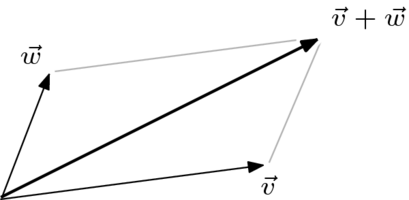
\includegraphics[width=0.4\linewidth]{optelling}
		\end{figure}
	\end{block} 
\end{frame}

\begin{frame}
	\frametitle{vectorspace}
	\begin{block}{First condition}
		A vectorspace V over a body L (set of operators) is a set of vectors that satisfy:\\
		1. A vectorsum is defined: $VxV\rightarrow V:(\overrightarrow{x},\overrightarrow{y})\rightarrow\overrightarrow{x}+\overrightarrow{y}$\\
		 \hspace{1.5 cm}$\overrightarrow{x}$, $\overrightarrow{y}$, $\overrightarrow{z}$ $\epsilon$ V
		\begin{description}
			\item[a)] $\overrightarrow{x}+\overrightarrow{y}$ $\epsilon$ V
			\item[b)] $\overrightarrow{x}+(\overrightarrow{y}+\overrightarrow{z})=(\overrightarrow{x}+\overrightarrow{y})+\overrightarrow{z}$
			\item[c)] $\exists!\overrightarrow{0}: \overrightarrow{x}+\overrightarrow{0}=\overrightarrow{0}+\overrightarrow{x}=\overrightarrow{x}$
			\item[d)] $\forall \overrightarrow{x}, \exists (-\overrightarrow{x}):\overrightarrow{x}+(-\overrightarrow{x})=(-\overrightarrow{x})+\overrightarrow{x}=0$
			\item[e)] $\overrightarrow{x}+\overrightarrow{y}=\overrightarrow{y}+\overrightarrow{x}$
		\end{description}
	\end{block}
\end{frame}

\begin{frame}
	\frametitle{vectorspace}
	\begin{block}{Second condition}
		2. A outside law is defined:$LxV\rightarrow V:(a,\overrightarrow{x})\rightarrow a\overrightarrow{x}$\\
		\hspace{1.5 cm}$\overrightarrow{x}$, $\overrightarrow{y}$ $\epsilon$ V\\
		\hspace{1.5 cm}a,b $\epsilon$ L
		\begin{description}
			\item[a)] $1\overrightarrow{x}=\overrightarrow{x}$
			\item[b)] $a(b\overrightarrow{x})=(ab)\overrightarrow{x}$
			\item[c)] $(a+b)\overrightarrow{x}=a\overrightarrow{x}+b\overrightarrow{x}$
			\item[d)] $a(\overrightarrow{x}+\overrightarrow{y})=a\overrightarrow{x}+a\overrightarrow{y}$
		\end{description}
	\end{block} 
\end{frame}

\begin{frame}
	\frametitle{Numberspaces of n-couples}
	\begin{block}{Defenition}
		This is the set of all n-couples like 
		$\begin{bmatrix}
			\overrightarrow{x_1}\\
			\overrightarrow{x_2}\\
			.\\
			.\\
			\overrightarrow{x_n}
		\end{bmatrix}$ with $x_i$ $\epsilon$ $\mathbb{R}$ or $x_i$ $\epsilon$ $\mathbb{C}$.\\
		This set together with the operator set $\mathbb{R}$ or $\mathbb{C}$ is a vectorspace.
	\end{block}
\end{frame}
		
\begin{frame}
	\frametitle{Subspaces}
	\begin{block}{Defenition}
		$V_1$ is a supspace of vectorspace V if:\\ 
		\begin{enumerate}
			\item $V_1 \subset$ V
			\item With the same in- and outside law as V, is $V_1$ a vectorspace
		\end{enumerate}
	\end{block}
	\begin{block}{Properties}
		\begin{enumerate}
			\item $\overrightarrow{0}$ $\epsilon$ every subspace
			\item The intersection of two spaces is always a subspace
			\item Given: p vectors $x_1,x_2,...,x_p$ $\epsilon$ V.\\
			The set vectors $a_1x_1+a_2x_2+...+a_nx_n$ with $a_i$ $\epsilon$ $\mathbb{R}$ is a subspace of V.
		\end{enumerate}
	\end{block}
\end{frame}

\begin{frame}
	\frametitle{Linear independance, basis, dimensions}
	\begin{block}{Defenition independance}
		Given: p vectors $\overrightarrow{x_1},\overrightarrow{x_2},...,\overrightarrow{x_p}$ $\epsilon$ V.\\
		Construct the nullvector as a linear combination of those vectors (i.e. search the operators (numbers) $a_1,a_2,...,a_p$ to form $a_1\overrightarrow{x_1}+a_2\overrightarrow{x_2}+...+a_n\overrightarrow{x_n}=\overrightarrow{0}$).\\
		If the nullvector only can created by $a_1=a_2=...=a_p=0$, then are the vectors $\overrightarrow{x_1},\overrightarrow{x_2},...,\overrightarrow{x_p}$ {\bf linear independant}.
	\end{block}
\end{frame}

\begin{frame}
	\frametitle{Linear independance, basis, dimensions}
	\begin{block}{Properties}
		\begin{enumerate}
			\item If the vectors $\overrightarrow{x_1},\overrightarrow{x_2},...,\overrightarrow{x_p}$ are linear independent, then can't none of them be writed as a linear combination of the other p-1 vectors.
			\item If the nullvector is one of the p vectors, then is the set $\overrightarrow{x_1},\overrightarrow{x_2},...,\overrightarrow{x_p}$ linear dependant (if $\overrightarrow{x_1}=0$ then is $a_1\overrightarrow{x_1}+a_2\overrightarrow{x_2}+...+a_n\overrightarrow{x_n}=0$ with $a_1\neq0$ and $a_2,a_3,...a_p=0$).
			\item Basis and dimension: p linear independant vectors $\overrightarrow{x_1},\overrightarrow{x_2},...,\overrightarrow{x_p}$ generate a vectrospace $V^p$. Every vector in $V^p$ can be writed {\bf in only one way} as a linear combination of the p linear independant vectors $\overrightarrow{x_1},\overrightarrow{x_2},...,\overrightarrow{x_p}$ using operators $a_1,a_2,...,a_p$.
		\end{enumerate}
	\end{block}
\end{frame}

\begin{frame}
	\frametitle{Linear independance, basis, dimensions}
	\begin{block}{Basis, dimension}
		Given: $\overrightarrow{v}=a_1\overrightarrow{x_1}+a_2\overrightarrow{x_2}+...+a_p\overrightarrow{x_p}$.\\
		The set operators $a_1,a_2,...,a_p$ are called the {\bf coordinates} of the vector $\overrightarrow{v}$ relative to the set vectors $\overrightarrow{x_1},\overrightarrow{x_2},...,\overrightarrow{x_p}$. This set vectors is a {\bf basis} of vectorspace $V^p$, with {\bf dimension} p.
	\end{block}
\end{frame}

\begin{frame}
	\frametitle{Linear independance, basis, dimensions}
	\begin{block}{Example}
		Given: $\overrightarrow{x_1}=\begin{bmatrix} 1\\0\\0\end{bmatrix}, \overrightarrow{x_2}=\begin{bmatrix} 0\\1\\0\end{bmatrix}, \overrightarrow{x_3}=\begin{bmatrix} 0\\0\\1\end{bmatrix}$\\
		The set \big\{$\overrightarrow{x_1},\overrightarrow{x_2},\overrightarrow{x_3}$\big\} is a linear independant combination. There doesn't exist numbers $a_1\neq0$, $a_2\neq0$, $a_3\neq0$ such that $a_1\overrightarrow{x_1}+a_2\overrightarrow{x_2}+a_n\overrightarrow{x_3}=0$. The set of all vectors $\overrightarrow{y}= a_1\overrightarrow{x_1}+ a_2\overrightarrow{x_2}+ a_n\overrightarrow{x_3}$ is the three dimensional vectrospace $V^3$.\\
		If $\overrightarrow{y}=\begin{bmatrix} 3\\2\\1\end{bmatrix}$. Then is $3\overrightarrow{x_1}+2\overrightarrow{x_2}+\overrightarrow{x_3}$ the only way to write $\overrightarrow{y}$ as a linear combination of $\overrightarrow{x_1},\overrightarrow{x_2},\overrightarrow{x_3}$.
	\end{block}
\end{frame}

\begin{frame}
	\frametitle{Linear independance, basis, dimensions}
	\begin{block}{Example}
		The set of vectors $\overrightarrow{y}=a_1\overrightarrow{x_1}+a_2\overrightarrow{x_2}$ is a {\bf two dimensional} subspace $V^2$.\\
		The vectors in this subspace are: $\overrightarrow{y}=\begin{bmatrix} y_1\\y_2\\y_3\end{bmatrix}=a_1\begin{bmatrix} 1\\0\\0\end{bmatrix}+ a_2\begin{bmatrix} 0\\1\\0\end{bmatrix}=\begin{bmatrix} a_1\\a_2\\0\end{bmatrix}$.
	\end{block}
	\begin{block}{Important difference}
		\begin{itemize}
			\item All vectors of $V^2$ have \textbf{3} coordinates.
			\item The dimension of the subspace $V^2$ is \textbf{2}.
		\end{itemize}
	\end{block}
\end{frame}

\begin{frame}
	\frametitle{Linear independance, basis, dimensions}
	\begin{block}{Convention of notation}
		Given: a n-dimensional vectorspace $V^n$.\\
		The elements of this vectorspace are the elements: $\overrightarrow{x},\overrightarrow{y},..$. If we choose $\overrightarrow{e_1},\overrightarrow{e_2},...,\overrightarrow{e_n}$ as a basis of $V^n$. Then we can write every vector of $V^n$ as a linear combination of those basis vectors in only one way: $\overrightarrow{x}=x_1\overrightarrow{e_1}+x_2\overrightarrow{e_2}+ ...+x_n\overrightarrow{e_n}$. The numbers $x_i$ are the coordinates of vector $\overrightarrow{x}$ relative to the basis $\overrightarrow{e_1},\overrightarrow{e_2},..., \overrightarrow{e_n}$.\vspace{5mm}
		Between the vectorspace of dimension n and the number space of dimension n exists a isomorphism.	
	\end{block}
\end{frame}

\begin{frame}
	\frametitle{Linear independance, basis, dimensions}
	\begin{block}{Vectorspace $V^p$}
		Given: a p-dimensional vectorspace $V^p$ where the vectors are n-couples (with $n\geq p$).
		\begin{enumerate}
			\item In $V^p$ you can choose a basis with p linear independant vectors.
			\item Every vector $\overrightarrow{x}$ $\epsilon$ $V^p$ can be writed in only one way as a linear combination of the p basis vectors using coordinates.
		\end{enumerate}	
	\end{block}
	\begin{block}{Example 1}
		Given: n=5, p=2, $\overrightarrow{x_1}=\begin{bmatrix} 1\\0\\-1\\2\\5\end{bmatrix}, \overrightarrow{x_2}=\begin{bmatrix} 2\\-3\\1\\0\\0\end{bmatrix}$.\\
	\end{block}
\end{frame}

\begin{frame}
	\frametitle{Linear independance, basis, dimensions}
	\begin{block}{Example 1}
		The vectors $\overrightarrow{x_1}$ and $\overrightarrow{x_2}$ are linear independant, so they span a two dimensional subspace: $\overrightarrow{y}=a_1\overrightarrow{x_1}+a_2\overrightarrow{x_2}$ with $a_1, a_2$ $\epsilon$ $\mathbb{R}$.\\
		The coordinates of the vector $y_1=\begin{bmatrix} 5\\-6\\1\\2\\5\end{bmatrix}$, relative to the basis \big\{$\overrightarrow{x_1},\overrightarrow{x_2}$\big\}, are $a_1=1$ and $a_2=2$.
	\end{block}
\end{frame}

\begin{frame}
	\frametitle{Linear independance, basis, dimensions}
	\begin{block}{Example 1}
		The vector $\overrightarrow{y_2}=\begin{bmatrix} 5\\-7\\1\\2\\5\end{bmatrix}$ can't be writen as a linear combination of the vectors $\overrightarrow{x_1}$ and $\overrightarrow{x_2}$. So $y_2$ doesn't belong to the subspace spanned by $\overrightarrow{x_1}$ and $\overrightarrow{x_2}$.\\
		This implies that $\overrightarrow{y_2}$ is linear independant of $\overrightarrow{x_1}$ and $\overrightarrow{x_2}$. Thus the subspace spanned by $\overrightarrow{y_2}$, $\overrightarrow{x_1}$ and $\overrightarrow{x_2}$ is a 3 dimensional subspace.
	\end{block}
\end{frame}

\begin{frame}
	\frametitle{Linear independance, basis, dimensions}
	\begin{block}{In general}
		When the set vectors $\overrightarrow{x_1},\overrightarrow{x_2},..., \overrightarrow{x_p}$ is linear independant, then lays $\overrightarrow{x_i}$ not totally in the subspace spanned by the vectors $\overrightarrow{x_1},..., \overrightarrow{x}_{i-1}, \overrightarrow{x}_{i+1},...,\overrightarrow{x_p}$.\\
		The vector $\overrightarrow{x_i}$ can be writen as a sum of 2 components: $\overrightarrow{x}_{i\alpha}$ and $\overrightarrow{x}_{i\beta}$.
		\begin{enumerate}
			\item $\overrightarrow{x}_{i\alpha}$ $\epsilon$ subspace spanned by $\overrightarrow{x_1},..., \overrightarrow{x}_{i-1}, \overrightarrow{x}_{i+1},...,\overrightarrow{x_p}$.
			\item $\overrightarrow{x}_{i\beta}$ $\bot$ subspace spanned by $\overrightarrow{x_1},..., \overrightarrow{x}_{i-1}, \overrightarrow{x}_{i+1},...,\overrightarrow{x_p}$.
		\end{enumerate}
	\end{block}
\end{frame}

\begin{frame}
	\frametitle{Inproduct}
	\begin{block}{Defenition}
		The inproduct of two vectors $\overrightarrow{x}$ and $\overrightarrow{y}$ $\epsilon$ $E^n$ (n-couples) is defined as the image: $E^nxE^n\to\mathbb{R}:\{\overrightarrow{x},\overrightarrow{y}\}\to\overrightarrow{x}.\overrightarrow{y}$ $\epsilon$ $\mathbb{R}$. This image is:
		\begin{enumerate}
			\item Bilinear:\\ $(\overrightarrow{x}+\overrightarrow{v}).\overrightarrow{y}=\overrightarrow{x}.\overrightarrow{y}+\overrightarrow{v}.\overrightarrow{y}$\\
			$\overrightarrow{x}+(\overrightarrow{v}).\overrightarrow{y})=\overrightarrow{x}.\overrightarrow{v}+\overrightarrow{x}.\overrightarrow{y}$\\
			$(a\overrightarrow{x})\overrightarrow{y}=a(\overrightarrow{x}.\overrightarrow{y})$\\
			$\overrightarrow{x}(a\overrightarrow{y})=a(\overrightarrow{x}.\overrightarrow{y})$
			\item Symetric:\\
			$\overrightarrow{x}.\overrightarrow{y}=\overrightarrow{y}.\overrightarrow{x}$
			\item Positive definite:\\
			$\forall \overrightarrow{x} \neq \overrightarrow{0}$: $\overrightarrow{x} .\overrightarrow{x} > 0$
		\end{enumerate}
	\end{block}
\end{frame}

\begin{frame}
	\frametitle{Inproduct}
	\begin{block}{Matricial notation}
		The inproduct is a {\bf scalar}. If $\overrightarrow{x}$, $\overrightarrow{y}$ and the basis $\epsilon$ $E^n$ then can the inproduct be noted matricial:\\
		$\overrightarrow{x}.\overrightarrow{y}=y^tAx=x^tAy=(x_1...x_n)A\begin{pmatrix} y_1\\...\\y_n\end{pmatrix}$\\
		with A positive definite and symetric ($A=A^t$).
	\end{block} 
\end{frame}

\begin{frame}
	\frametitle{Inproduct}
	\begin{block}{Norm of a vector}
		$\|\overrightarrow{x}\|^2=\overrightarrow{x}.\overrightarrow{x}$ and because $\overrightarrow{x}.\overrightarrow{x}>0$ applies:\\
		$\|\overrightarrow{x}\|=\sqrt{\overrightarrow{x}.\overrightarrow{x}}$ where $\|\overrightarrow{x}\|$ is called the norm of $\overrightarrow{x}$.\\
		Normalizing is dividing a vector by its norm. The result is a vector with norm $=1$.\\
		$\|\frac{\overrightarrow{x}}{\|\overrightarrow{x}\|}\|= \sqrt{\frac{\overrightarrow{x}}{\|\overrightarrow{x}\|} \frac{\overrightarrow{x}}{\|\overrightarrow{x}\|}}= \sqrt{\frac{\|\overrightarrow{x}\|^2}{\|\overrightarrow{x}\|\|\overrightarrow{x}\|}}=1$.
	\end{block} 
\end{frame}

\begin{frame}
	\frametitle{Inproduct}
	\begin{block}{Cauchy–Schwarz inequality}
		$|\overrightarrow{x}.\overrightarrow{y}|\leq \|\overrightarrow{x}\|\|\overrightarrow{y}\|$ or \\
		$-\|\overrightarrow{x}\|\|\overrightarrow{y}\|\leq \overrightarrow{x}.\overrightarrow{y}\leq \|\overrightarrow{x}\|\|\overrightarrow{y}\|$ from wich follows:\\
		$-1 \leq\frac{\overrightarrow{x}\overrightarrow{y}} {\|\overrightarrow{x}\|\|\overrightarrow{y}\|} \leq 1$\\
		By defenition follows:\\
		$\cos(\theta)=cos(\angle (\overrightarrow{x}, \overrightarrow{y}))= \frac{\overrightarrow{x}\overrightarrow{y}} {\|\overrightarrow{x}\|\|\overrightarrow{y}\|}$\\
		Therefor: the angle between the vectors $\overrightarrow{x}$ and $\overrightarrow{y}$ = Bgcos(inproduct of $\frac{\overrightarrow{x}}{\|\overrightarrow{x}\|}$ and $\frac{\overrightarrow{y}}{\|\overrightarrow{y}\|}$).
	\end{block} 
\end{frame}

\begin{frame}
	\frametitle{Inproduct}
	\begin{block}{Orthogonality}
		$\overrightarrow{x}$ and $\overrightarrow{y}$ are orthogonal $\Leftrightarrow$\\ $\theta=\angle(\overrightarrow{x},\overrightarrow{y})=90^{\circ}=\frac{\Pi}{2} rad$ $\Leftrightarrow$\\
		$cos(\theta)=0$ $\Leftrightarrow$\\
		$\overrightarrow{x}.\overrightarrow{y}=0$\\
		\vspace{5mm}
		Hence, if $\overrightarrow{x},\overrightarrow{y} \neq 0$:\\
		$\overrightarrow{x}\perp\overrightarrow{y} \Leftrightarrow \overrightarrow{x}.\overrightarrow{y}=0$.
	\end{block} 
	\begin{block}{Parallellism}
		$\overrightarrow{x}\parallel\overrightarrow{y}\Leftrightarrow
		\theta=0^{\circ}$ or $180^{\circ} \Leftrightarrow
		cos(\theta)=\pm 1 \Leftrightarrow
		|\overrightarrow{x}\overrightarrow{y}|=\|\overrightarrow{x}\|\|\overrightarrow{y}\|$
	\end{block} 
\end{frame}

\begin{frame}
	\frametitle{Inproduct}
	\begin{block}{Distance between two vectors}
		Distance $=\|\overrightarrow{x}-\overrightarrow{y}\|=\|\overrightarrow{z}\|$ with $\overrightarrow{z}=\overrightarrow{x}-\overrightarrow{y}$.\\
		$\|\overrightarrow{x}-\overrightarrow{y}\|^2=(\overrightarrow{x}-\overrightarrow{y}) (\overrightarrow{x}-\overrightarrow{y})$ \\
		$=\overrightarrow{x}\overrightarrow{x}-\overrightarrow{x}\overrightarrow{y}-\overrightarrow{y}\overrightarrow{x}+\overrightarrow{y}\overrightarrow{y}$ \\ 
		$=\overrightarrow{x}\overrightarrow{x}+\overrightarrow{y}\overrightarrow{y}-2\overrightarrow{x}\overrightarrow{y}$ \\
		$=\|\overrightarrow{x}\|^2+\|\overrightarrow{y}\|^2-2\|\overrightarrow{x}\|\|\overrightarrow{y}\|cos(\theta)$ with $\theta$ the angle between $\overrightarrow{x}$ and $\overrightarrow{y}$.
	\end{block}
	\begin{block}{Pythagorean theorem}
		If $\overrightarrow{x}\perp\overrightarrow{y}$ then $cos(\theta)=0$ and thus:\\
		$\|\overrightarrow{x}-\overrightarrow{y}\|^2=\|\overrightarrow{x}\|^2+\|\overrightarrow{y}\|^2$.
	\end{block} 
\end{frame}

\begin{frame}
	\frametitle{Inproduct}
	\begin{block}{The 'simple' inproduct}
		If in the definition $\overrightarrow{x}.\overrightarrow{y}=y^tAx=x^tAy$ 
		(with A positive definite and symetric) A=I, then the inproduct becomes the simple inproduct: $\overrightarrow{x}.\overrightarrow{y}=y^tIx=x^tIy=(x_1...x_n)\begin{pmatrix} y_1\\...\\y_n\end{pmatrix}=\sum_{i=1}^{n}x_iy_i$.\\
		This simple inproduct can always be found by a basis transformation: x=Rx' and y=Ry', then $\overrightarrow{x}.\overrightarrow{y}=y'^t(R^tAR)x'$.\\
		Now, R must be taken such that $R^tAR=I$. This can be done by converting A to its normal form by a congruent transformation (e.g. the method of kwadratic forms). \\
		\vspace{5mm}
		In what follows we mean by 'inproduct' always 'simple inproduct'.
	\end{block} 
\end{frame}

\begin{frame}
	\frametitle{Gram Schmidt orthogonalization}
	\begin{block}{Making two independent vectors orthogonal}
		Geometric derivation:
		\begin{columns}
			\begin{column}{.49\textwidth}
				\setlength{\unitlength}{1mm}
				\begin{picture}(60,40)
					\put(15, 10){\vector(1,0){40}}
					\put(55, 4){$\overrightarrow{x}$}
					\put(15, 10){\vector(1,1){25}}
					\put(30, 31){$\overrightarrow{y}$}	
					\put(20,11){$\theta$}	
					\put(15,10){\vector(1,0){25}}	
					\put(15,10){\vector(0,1){25}}
					\put(40,4){$\overrightarrow{y_1}$}
					\put(10,35){$\overrightarrow{y_2}$}			
				\end{picture}
			\end{column}
			\begin{column}{.49\textwidth}
				Figure 1: decomposition of vector $\overrightarrow{y}$ in a component parallel ($\overrightarrow{y_1}$) and a component orthogonal ($\overrightarrow{y_2}$) to $\overrightarrow{x}$.
			\end{column}	
		\end{columns}
	\end{block} 
\end{frame}

\begin{frame}
	\frametitle{Gram Schmidt orthogonalization}
	\begin{block}{Making two indepentent vectors orthogonal}
		\begin{enumerate}
			\item Project $\overrightarrow{y}$ orthogonal on $\overrightarrow{x}$, this generates the vector $\overrightarrow{y_1}$, the component parallel with $\overrightarrow{x}$.
			\item Subtract $\overrightarrow{y}$ by $\overrightarrow{y_1}$, the result is $\overrightarrow{y_2}$ wich is orthogonal to $\overrightarrow{x}$.
		\end{enumerate}
		$\overrightarrow{y_1}$ is a specific multiple of the normilised vector $\overrightarrow{x}$:
		$\overrightarrow{y_1}=\alpha\frac{\overrightarrow{x}}{\|\overrightarrow{x}\|}$.\\
		$\overrightarrow{y_1}\parallel\overrightarrow{x}$: $\overrightarrow{y_1}\overrightarrow{x}=\pm\|\overrightarrow{y_1}\|\|\overrightarrow{x}\|$ (+ if $\theta\leq90^{\circ}$ and - if $\theta>90^{\circ}$).\\
		From fig. 1: $\|\overrightarrow{y_1}\|=cos(\theta)\|\overrightarrow{y}\|$.\\
		From the inproduct: $cos(\theta)=\frac{\overrightarrow{x}\overrightarrow{y}}{\|\overrightarrow{x}\|\|\overrightarrow{y}\|}$.
		So $\overrightarrow{y_1}\overrightarrow{x}=\alpha\frac{\overrightarrow{x}}{\|\overrightarrow{x}\|}\overrightarrow{x}=\alpha\|\overrightarrow{x}\|=\|\overrightarrow{y_1}\|\|\overrightarrow{x}\|=cos(\theta)\|\overrightarrow{y}\|\|\overrightarrow{x}\|=\overrightarrow{x}\overrightarrow{y}$.\\
		So we get: $\alpha=\frac{\overrightarrow{x}\overrightarrow{y}}{\|\overrightarrow{x}\|}$.
	\end{block} 
\end{frame}

\begin{frame}
	\frametitle{Gram Schmidt orthogonalization}
	\begin{block}{Conclusion}
		$\overrightarrow{y_1}=\alpha\frac{\overrightarrow{x}}{\|\overrightarrow{x}\|}=(\frac{\overrightarrow{x}\overrightarrow{y}}{\|\overrightarrow{x}\|^2})\overrightarrow{x}$ with $\frac{\overrightarrow{x}\overrightarrow{y}}{\|\overrightarrow{x}\|^2}$ a scalar.\\
		And $\overrightarrow{y_2}=\overrightarrow{y}-\overrightarrow{y_1}=\overrightarrow{y}-(\frac{\overrightarrow{x}\overrightarrow{y}}{\|\overrightarrow{x}\|^2})\overrightarrow{x}$.\\
		Hence:
		\fbox{
			\begin{minipage}{10cm}{The vector $\overrightarrow{y}$ gets orthogonalised on the vector $\overrightarrow{x}$ by subtract $\overrightarrow{y}$ by the component of $\overrightarrow{y}$ parallel with $\overrightarrow{x}$}.
			\end{minipage}
		}
		Control of $\overrightarrow{y_2}\perp\overrightarrow{x}$:\\
		$\overrightarrow{y_2}\overrightarrow{x}=(\overrightarrow{y}-(\frac{\overrightarrow{x}\overrightarrow{y}}{\|\overrightarrow{x}\|^2})\overrightarrow{x})\overrightarrow{x}=\overrightarrow{y}\overrightarrow{x}-(\frac{\overrightarrow{x}\overrightarrow{y}}{\|\overrightarrow{x}\|^2})\|\overrightarrow{x}\|^2=0$.
	\end{block} 
\end{frame}

\begin{frame}
	\frametitle{Gram Schmidt orthogonalization}
	\begin{block}{Generalization to multiple vectors}
		Given: 3 vectors: 2 orthogonal unit vectors $\overrightarrow{x_1}$ and $\overrightarrow{x_2}$ ($\|\overrightarrow{x_1}\|=1=\|\overrightarrow{x_2}\|,\overrightarrow{x_1}\overrightarrow{x_2}=0)$ and a vector $\overrightarrow{y}$.\\
		Asked: orthogonilise $\overrightarrow{y}$ on $\overrightarrow{x_1}$ and $\overrightarrow{x_2}$.\\
		Solution:\\
		We first search the component of $\overrightarrow{y}$ parallel with $\overrightarrow{x_1}$ and subtract $\overrightarrow{y}$ by this component. This gives $\overrightarrow{y_1}$.\\
		$\overrightarrow{y_1}=\overrightarrow{y}-(\frac{\overrightarrow{x_1}\overrightarrow{y}}{\|\overrightarrow{x_1}\|^2})\overrightarrow{x_1}=\overrightarrow{y}-(\overrightarrow{x_1}\overrightarrow{y})\overrightarrow{x_1}$ ($\|\overrightarrow{x_1}\|^2=1$)\\
		$\overrightarrow{y_1}\perp\overrightarrow{x_1}$.
	\end{block} 
\end{frame}

\begin{frame}
	\frametitle{Gram Schmidt orthogonalization}
	\begin{block}{Generalization to multiple vectors}
		Next, we subtract $\overrightarrow{y_1}$ by the component of $\overrightarrow{y_1}$ that is parallel with $\overrightarrow{x_2}$, to get $\overrightarrow{z}$ (wich is perpendicular to both $\overrightarrow{x_1}$ and $\overrightarrow{x_2}$).\\
		$\overrightarrow{z}=\overrightarrow{y_1}-\overrightarrow{x_2}(\overrightarrow{y_1}\overrightarrow{x_2})$. We can write $\overrightarrow{z}$ in another way:\\
		$\overrightarrow{z}=\overrightarrow{y_1}-\overrightarrow{x_2}(\overrightarrow{y_1}\overrightarrow{x_2})=\overrightarrow{y}-(\overrightarrow{x_1}\overrightarrow{y})\overrightarrow{x_1}-\overrightarrow{x_2}([\overrightarrow{y}-(\overrightarrow{x_1}\overrightarrow{y})\overrightarrow{x_1}]\overrightarrow{x_2})$\\
		$\overrightarrow{z}=\overrightarrow{y}-\overrightarrow{x_1}(\overrightarrow{x_1\overrightarrow{y}})-\overrightarrow{x_2}(\overrightarrow{x_2}\overrightarrow{y})$
	\end{block} 
	\begin{block}{Conclusion}
		The vector $\overrightarrow{y}$ becomes orthogonilised on two orthogonal unit vectors $\overrightarrow{x_1}$ and $\overrightarrow{x_2}$ by subtracting $\overrightarrow{y}$ by the components of $\overrightarrow{y}$ parallel with $\overrightarrow{x_1}$ and $\overrightarrow{x_2}$.
	\end{block}
\end{frame}

\begin{frame}
	\frametitle{Complementary subspace}
	\begin{block}{Defenition}
		Given: a n dimensional vector space $V^n$, with $p<n$ linear independent vectors $\overrightarrow{x_1},\overrightarrow{x_2},...,\overrightarrow{x_p}$. This vectors create a p dimensional subspace $V^p$ and can be orthogonilised via the Gram schidt method to a orthonormal basis $\overrightarrow{e_1},\overrightarrow{e_2},...,\overrightarrow{e_p}$ with $\overrightarrow{e_i}\overrightarrow{e_j}=\delta_{ij}$ (with $\delta_{ij}=1$ if $i=j$ and $\delta_{ij}=0$ if $i\neq j$).\\
		This p vectors can be complemented by $n-p$ linear independent vectors $\overrightarrow{f_1},\overrightarrow{f_2},...,\overrightarrow{f_{n-p}}$ that are linear independent with $\overrightarrow{e_1},\overrightarrow{e_2},...,\overrightarrow{e_p}$ and orthonormal.\\
		\vspace{4mm}
		These vectors $\overrightarrow{f_1},\overrightarrow{f_2},...,\overrightarrow{f_{n-p}}$ generate the orthogonal complement of the subspace created by $\overrightarrow{e_1},\overrightarrow{e_2},...,\overrightarrow{e_p}$. \\
		The orthogonal complement of the p-dimensional subspace $V^p$ of $V^n$ ($p<n$), has dimension $n-p$.
	\end{block}
\end{frame}
					
\begin{frame}
	\frametitle{Complementary subspace}
	\begin{block}{Example}
		Given: $n=5,p=3, \overrightarrow{e_1}=\begin{bmatrix} 2\\0\\-1\\0\\0 \end{bmatrix}, \overrightarrow{e_2}=\begin{bmatrix} 1\\0\\0\\4\\0 \end{bmatrix}, \overrightarrow{e_3}=\begin{bmatrix} 1\\3\\1\\0\\0 \end{bmatrix}$.\\
		Asked: The orthogonal complement\\
		Solution: The orthogonal complement has dimension $n-p=5-3=2$ and consists of the set vectors that are perpendicular to the vectors $\overrightarrow{e_1},\overrightarrow{e_2},...,\overrightarrow{e_p}$.\\
		$\begin{cases}
			\overrightarrow{e_1}\overrightarrow{x}=0\\
			\overrightarrow{e_2}\overrightarrow{x}=0\\
			\overrightarrow{e_3}\overrightarrow{x}=0
		\end{cases}$
	\end{block}
\end{frame}

\begin{frame}
	\frametitle{Complementary subspace}
	\begin{block}{Example}
		$\begin{cases}
		\begin{bmatrix} 2 & 0 & -1 & 0 & 0 \end{bmatrix} \overrightarrow{x}=0\\
		\begin{bmatrix} 1 & 0 & 0 & 4 & 0 \end{bmatrix} \overrightarrow{x}=0\\
		\begin{bmatrix} 1 & 3 & 1 & 0 & 0 \end{bmatrix} \overrightarrow{x}=0
		\end{cases}$\\
		$\begin{bmatrix} 
		2 & 0 & -1 & 0 & 0\\
		1 & 0 & 0 & 4 & 0\\
		1 & 3 & 1 & 0 & 0
		\end{bmatrix} 
		\begin{bmatrix}
		\overrightarrow{x_1}\\ \overrightarrow{x_2}\\ \overrightarrow{x_3}\\ \overrightarrow{x_4}\\ \overrightarrow{x_5}
		\end{bmatrix}=0$\\
		This is a homogenous system of equetions. The solution of this system is the orthogonal complement. 	
	\end{block}
\end{frame}


\section{Matrices}

\begin{frame}
	\frametitle{Row- and column vectors}
	\begin{block}{Example}
		The rows of a mxn matrix A can be considered as m row vectors with n components.\\
		$A^{mxn}=\begin{bmatrix} \overrightarrow{r_1}\\ \overrightarrow{r_2}\\ ...\\\overrightarrow{r_m}\end{bmatrix}$\\
		The columns of a mxn matrix A can be considered as n column vectors with m components.\\
		$A^{mxn}=\begin{bmatrix} \overrightarrow{r_1}& \overrightarrow{r_2}& ...& \overrightarrow{r_m}\end{bmatrix}$
	\end{block}
\end{frame}

\begin{frame}
	\frametitle{Row- and column space, rank}
	\begin{block}{Column space}
		We consider the columns of $A^{mxn}$ as vectors with m components and difine the vectors $\overrightarrow{x}$ as every possible linear combination of the column vectors $\overrightarrow{k_i}$:\\
		$\overrightarrow{x}=a_1\overrightarrow{k_1}+a_2\overrightarrow{k_2}+...+a_n\overrightarrow{k_n}$ with $a_i\in\mathbb{R}$ and i means the $i^{th}$ column of A.\\
		The set of all the vectors $\overrightarrow{x}$ is called the column space of A.\\
		The column space = all possible linear combinations of columns of A .
		\end{block}
\end{frame}

\begin{frame}
	\frametitle{Row- and column space, rank}
	\begin{block}{Column space}
		if only r of the n vectors are linear independent, that means\\
		\begin{itemize}
			\item None of this r vectors can be written as a linear combination of the other $r-1$ vectors
			\item all others $n-r$ column vectors can be written as linear combinations of the r linear independant vectors
		\end{itemize} 
		then r is called:
		\begin{enumerate}
			\item the rank of (column) matrix A
 			\item the dimension of the column space of matrix A
		\end{enumerate}
	\end{block}
\end{frame}

\begin{frame}
	\frametitle{Row- and column space, rank}
	\begin{block}{Row space}
		The concept row space and row rank can be derived in the same way as the column space is derived.
	\end{block}
	\begin{block}{Rank}
		It is a fundamental matrix property that: $\framebox[1.1\width]{row rank A = column rank A}$\\
		That means: the number linear independant columns in a matrix is equal to the number linear independant rows. Thus: \\
		{rank A = row rank A = column rank A \par
		= dimension row space A = dimension column space A} 	
	\end{block}
\end{frame}

\begin{frame}
	\frametitle{Row- and column space, rank}
	\begin{block}{Example}
		$A^{4x3}=\begin{bmatrix} 1 & 2 & -1 \\ 0 & 1 & 0 \\ 1 & 3 & -1 \\ 2 & 4 & -2 \end{bmatrix}= \begin{bmatrix} k_1 & k_2 & k_3 \end{bmatrix}= \begin{bmatrix} r_1\\r_2\\r_3\\r_4
		\end{bmatrix}$ \\
		We determine the rank of A by converting it to his echlon form by elementary row operations (explaned in the appendix).\\
		$\begin{bmatrix} 1 & 2 & -1 \\ 0 & 1 & 0 \\ 1 & 3 & -1 \\ 2 & 4 & -2 \end{bmatrix} \sim \begin{bmatrix} 1 & 2 & -1 \\ 0 & 1 & 0 \\ 0 & 1 & 0 \\ 0 & 0 & 0 \end{bmatrix} \sim \begin{bmatrix} 1 & 0 & -1 \\ 0 & 1 & 0 \\ 0 & 0 & 0 \\ 0 & 0 & 0 \end{bmatrix}$\\
		Canonical form: the first element of every row is 1. Above and below this ones is every number 0.\\
	\end{block}
\end{frame}

\begin{frame}
	\frametitle{Row- and column space, rank}
	\begin{block}{Conclusion}
		Rank = the number of rows that differs from zero. So the rank is 2. In other words: there are only 2 linear independent rows and columns in A. \\
		Hence:\\
		The column space of A is a 2 dimensional subspace of the 4 dimensional vectorspace.\\
		The row space is a 2 dimensional subspace of the 3 dimensional space.
	\end{block}
\end{frame}

\begin{frame}
	\frametitle{Link between determinant and rank by square matrices}
	\begin{block}{Determinant-rank}
		If all the columns of a square matrix are linear dependent, then the determinant is 0. If $A^{mxm}$: \\
		det A=0 $\Leftrightarrow$ rank A=0 $\Leftrightarrow$ columns depentent $\Leftrightarrow$ rows dependent.
		If det A $\neq 0$ then rank A = m and A is of {\bf full rank}. A matrix can be inverted is his determinant when different from 0 (when its of full rank).
	\end{block}
\end{frame}

\begin{frame}
	\frametitle{Link between determinant and rank by square matrices}
	\begin{block}{Determinant-rank}
		If rank($B^{nxn}$)=r with r$\leq$n and rank($A^{nxn}$)=n (A is of full rank) then is:\\
		rank(AB)=rank(BA)=rank(B).\\
		Elementary row- and column operations are always of full rank (appendix). When there is a multiplication between a matrix and a elementary row- or column matrix, then has the product always the rank of the matrix.
	\end{block}
\end{frame}

\begin{frame}
	\frametitle{Column space test}
	\begin{block}{Belongs the vector to the column space?}
		Given: n vectors with m components relative to a basis in $V^m$:\\
		$\begin{bmatrix} x_{11}\\x_{21}\\...\\x_{m1} \end{bmatrix},...,\begin{bmatrix} x_{1n}\\x_{2n}\\...\\x_{nn}\end{bmatrix}$.\\
		If r of this n vectors are linear independent then has the matrix \\
		$X^{mxn}=\begin{bmatrix} \overrightarrow{x_1},...,\overrightarrow{x_n}\end{bmatrix}=\begin{bmatrix} x_{11} & ... & x_{1n}\\ ... & & ...\\ x_{m1} & ... & x_{mn}\end{bmatrix}$\\
		rank r. The column space of X has dimension r.
	\end{block}
\end{frame}

\begin{frame}
	\frametitle{Column space test}
	\begin{block}{Belongs the vector to the column space?}
		How can you determine of a given vector $\overrightarrow{y}$ with m components belongs to the column space of X?\\
		 If $\overrightarrow{y}$ is a element of the column space of X, then can $\overrightarrow{y}$ be written as a linear combination of the vectors $\overrightarrow{x_1},...,\overrightarrow{x_n}$. By adding $\overrightarrow{y}$ to this vectors, the spanned space will be the same and the rank will still be r. \\
		In other words, if $\overrightarrow{y}$ belongs to the column space of X, then will the rank of the expanded matrix $\begin{bmatrix} \overrightarrow{x_1},...,\overrightarrow{x_n},\overrightarrow{y}\end{bmatrix}$
		be the same as the rank of the normal matrix X.\\
		\vspace{4mm}
		\framebox[1.1\width]{$\overrightarrow{y}\in$ column space $\Leftrightarrow rank\begin{bmatrix}
		X & \overrightarrow{y} \end{bmatrix}=rank\begin{bmatrix}
		X \end{bmatrix} =r$}
	\end{block}
\end{frame}

\begin{frame}
	\frametitle{Column space test}
	\begin{block}{Vector $\overrightarrow{y}$ not in column space}
		If $\overrightarrow{y}$ doesn't belong to the column space of X, then can't $\overrightarrow{y}$ be written as a linear combination of the vectors $\overrightarrow{x_1},...,\overrightarrow{x_n}$, in other words: $\overrightarrow{y}$ can be splitted in two vectors $\overrightarrow{y}=\overrightarrow{z_1}+\overrightarrow{z_2}$ with $\overrightarrow{z_1}$ in the column space of X and $\overrightarrow{z_2}$ not in the column space of X. By adding $\overrightarrow{y}$ to the vectors $\overrightarrow{x_1},...,\overrightarrow{x_n}$ increases the dimension of the spannend space.\\
		\vspace{4mm}
		\framebox[1.1\width]{$\overrightarrow{y}\not\in$ column space $\Leftrightarrow rank\begin{bmatrix}
		X & \overrightarrow{y} \end{bmatrix}=r+1$}\\
	\vspace{4mm}
	{\bf Remark:} rank$\begin{bmatrix} X & \overrightarrow{z_1} \end{bmatrix} =r$ and rank$\begin{bmatrix} X & \overrightarrow{z_2} \end{bmatrix} =r+1$.
	\end{block}
\end{frame}

\begin{frame}
	\frametitle{Column space test}
	\begin{block}{Resume}
		\begin{enumerate}
			\item n vectors with m components $\overrightarrow{x_1},...,\overrightarrow{x_n}$
			\item Belongs $\overrightarrow{y}$ to the space spanned by $\overrightarrow{x_1},...,\overrightarrow{x_n}$?
			\item Solution:
				\begin{description}
					\item[a)] Determine $r_1=rank\begin{bmatrix} X\end{bmatrix}=rank\begin{bmatrix} \overrightarrow{x_1} & ... & \overrightarrow{x_n} \end{bmatrix}$
					\item[b)] Determine $r_2=rank\begin{bmatrix} X & \overrightarrow{y}\end{bmatrix}=rank\begin{bmatrix} \overrightarrow{x_1} & ... & \overrightarrow{x_n} & \overrightarrow{y} \end{bmatrix}$
					\item[c)] Is $r_1=r_2 \Rightarrow y\in$ column space or $r_1+1=r_2 \Rightarrow y\not\in$ column space
				\end{description}
		\end{enumerate}
		\vspace{2mm}
		{\bf Remark}: analogous for the row space test.
	\end{block}
\end{frame}

\begin{frame}
	\frametitle{Column space test}
	\begin{block}{Example}
		Given: $\overrightarrow{x_1}=\begin{bmatrix} 1\\2\\3\\4\\5\end{bmatrix}, \overrightarrow{x_2}=\begin{bmatrix} -1\\2\\0\\5\\7\end{bmatrix}, \overrightarrow{x_3}=\begin{bmatrix} 0\\4\\3\\9\\12\end{bmatrix}, \overrightarrow{y}=\begin{bmatrix} -1\\-1\\2\\1\\0\end{bmatrix}$\\
		Asked: Belongs $\overrightarrow{y}$ to the space spanned by $\overrightarrow{x_1},\overrightarrow{x_2},\overrightarrow{x_3}$?\\
		Solution: 1$)$ find the rang of X:\\
		$X=\begin{bmatrix}
			1 & -1 & 0\\
			2 & 2 & 4\\
			3 & 0 & 3\\
			4 & 5 & 9\\
			5 & 7 & 12\\\end{bmatrix}\sim\begin{bmatrix}
			1 & -1 & 0\\
			2 & 2 & 0\\
			3 & 0 & 0\\
			4 & 5 & 0\\
			5 & 7 & 0\\
			\end{bmatrix}\sim\begin{bmatrix}
				1 & 0 & 0\\
				0 & 1 & 0\\
				\frac{3}{2} & \frac{3}{4} & 0\\
				-\frac{1}{2} & \frac{9}{4} & 0\\
				-1 & \frac{12}{4} & 0\\
			\end{bmatrix}$\\ Hence, rank(X)$=2$.
	\end{block}
\end{frame}

\begin{frame}
	\frametitle{Column space test}
	\begin{block}{Example}
		2$)$ Determine the rank$\begin{bmatrix}
		X & \overrightarrow{y}\end{bmatrix}$\\
		$\begin{bmatrix}
		X & \overrightarrow{y}\end{bmatrix}=\begin{bmatrix} 
		1 & -1 & 0 & -1\\
		2 & 2 & 4 & -1\\
		3 & 0 & 3 & 2\\
		4 & 5 & 9 & 1\\
		5 & 7 & 12 & 0\\\end{bmatrix}$ \hspace{1cm} rank$\begin{bmatrix}
		X & \overrightarrow{y}\end{bmatrix}=3$.\\
		Hence, rank$\begin{bmatrix}
		X & \overrightarrow{y}\end{bmatrix}=rank\begin{bmatrix}
		X \end{bmatrix}+1$.\\
		That means: $\overrightarrow{y}$ can {\bf not} be written as a linear combination of the vectors $\overrightarrow{x_1},\overrightarrow{x_2},\overrightarrow{x_3}$ and doesn't belong to the space spanned by this vectors. Because rank(X)$=2$ is the dimension of the space 2. Hence $\overrightarrow{x_3}$ can be written as a linear combination of $\overrightarrow{x_1},\overrightarrow{x_2}$. Rank(X$\overrightarrow{y}$)=3, so the space spanned by $\overrightarrow{x_1},\overrightarrow{x_2},\overrightarrow{x_3}$ and $\overrightarrow{y}$ has dimension 3.
	\end{block}
\end{frame}

\begin{frame}
	\frametitle{Orthonormal matrices}
	\begin{block}{Definition}
		The set vectors $\overrightarrow{e_1},\overrightarrow{e_2},...,\overrightarrow{e_n}$ is orthonormal if:
		\begin{itemize}
			\item $\|\overrightarrow{e_i}\|=1$ with $i=1,...,n$
			\item $\overrightarrow{e_i}\perp\overrightarrow{e_j}$ or $\overrightarrow{e_i}.\overrightarrow{e_j}=0$ with $i\neq j$
		\end{itemize}
		This is noted as:\\
		$\overrightarrow{e_i}.\overrightarrow{e_j}=\delta_{ij}$ with $\delta_{ij}=0$ if $i\neq j$ and $\delta_{ij}=1$ if $i=j$ ($\delta_{ij}$ is called 'kronecker delta').\\
		If $\overrightarrow{e_{1i}}$ has the components $\begin{bmatrix} \overrightarrow{e_{1i}}\\...\\\overrightarrow{e_{ni}}\end{bmatrix}$ relative to some basis, then applies for the inproduct:\\
		$\overrightarrow{e_{1i}}.\overrightarrow{e_{1j}}=\begin{bmatrix} e_{1i} & ... & e_{ni}\end{bmatrix} \begin{bmatrix} e_{1i}\\...\\e_{ni}\end{bmatrix}=e_{1i}e_{1j}+...+e_{ni}e_{nj}=\delta_{ij}$
	\end{block}
\end{frame}

\begin{frame}
	\frametitle{Orthonormal matrices}
	\begin{block}{Defenition}
		If we create from $\overrightarrow{e_1},\overrightarrow{e_2},...,\overrightarrow{e_n}$ the matrix \\
		$E=\begin{bmatrix} \overrightarrow{e_1},...,\overrightarrow{e_n}\end{bmatrix}=\begin{bmatrix} 
		e_{11} & ... & e_{1n}\\
		... & & ...\\
		e_{n1} & ... & e_{nn}\end{bmatrix}$ \\
		then applies\\
		$E^tE=\begin{bmatrix} 
		e_{11} & ... & e_{n1}\\
		... & & ...\\
		e_{1n} & ... & e_{nn}\end{bmatrix}\begin{bmatrix} 
		e_{11} & ... & e_{1n}\\
		... & & ...\\
		e_{n1} & ... & e_{nn}\end{bmatrix}=\begin{bmatrix} 
		1 & 0 & ... & 0\\
		0 & 1 & ... & 0\\
		... & ... & ... & ...\\
		0 & 0 & ... & 1\end{bmatrix}=I^{nxn}$\\
		Hence, if the columns and rows of a matrix form a orthonomal system then is the matrix onthonormal: $E^tE=I=EE^t$.
	\end{block}
\end{frame}

\begin{frame}
	\frametitle{Orthonormal matrices}
	\begin{block}{Properties}
		\begin{enumerate}
			\item The inverse of a orthonormal matrix is his transform:\\
			$E^tE=I=EE^t \Rightarrow E^{-1}EE^t=E^{-1}I \Rightarrow IE^t=E^{-1} \Rightarrow E^t=E^{-1}$
			\item Maintaining the norm of a vector: $\overrightarrow{x}$ is a vector with norm $\|\overrightarrow{x}\|$ and E an orthonormal matrix then applies $\|E\overrightarrow{x}\|=\|\overrightarrow{x}\|$.\\
			When there is a 'fault' $\Delta x$ on x, then is $\|E(\overrightarrow{x}+\Delta\overrightarrow{x})\|=\|\overrightarrow{x}+\Delta\overrightarrow{x}\|$.\\
			Hence, an orthogonal matrix doesn't change the magnitude of a fault. This is important in numerical applications.
			\item The determinant of an orthonormal matrix is $\pm1$, when it is 1 the matrix represent a rotation matrix.
		\end{enumerate}
	\end{block}
\end{frame}

\begin{frame}
	\frametitle{Change of basis and matrix representation}
	\begin{block}{Change of basis}
		In a n dimension vectorspace $V^n$ are two different bases given:\\
		'old basis': $\overrightarrow{e_1},....,\overrightarrow{e_n}$\\
		'new basis': $\overrightarrow{f_1},...,\overrightarrow{f_n}$\\
		A vector x has coordinates $\begin{bmatrix} a_1\\...\\a_n\end{bmatrix}$ relative to the old basis and coordinates $\begin{bmatrix} b_1\\...\\b_n\end{bmatrix}$ relative to the new basis.
	\end{block}
\end{frame}

\begin{frame}
	\frametitle{Change of basis and matrix representation}
	\begin{block}{Change of basis}
		Every basisvector $\overrightarrow{f_i}$ can be expressed as a linear combination of the old basis vectors:$\overrightarrow{f_i}=f_{1i}\overrightarrow{e_1}+...+f_{ni}\overrightarrow{e_n}$. So $\overrightarrow{f_i}$ has coordinates $\begin{bmatrix} f_{1i}\\...\\f_{ni}
		\end{bmatrix}$ relative to the old basis.\\
		If we group the old basis vectors in a matrix:
		$E=\begin{bmatrix} \overrightarrow{e_1} & ... & \overrightarrow{e_n} \end{bmatrix}$ then you can write: $\overrightarrow{x}=\begin{bmatrix} \overrightarrow{e_1} & ... & \overrightarrow{e_n} \end{bmatrix} \begin{bmatrix} a_1 \\ ... \\ a_n \end{bmatrix}=E\overrightarrow{x}_{old}$ and $\overrightarrow{f_i}=\begin{bmatrix} \overrightarrow{e_1} & ... & \overrightarrow{e_n} \end{bmatrix} \begin{bmatrix} f_{1i} \\ ... \\ f_{ni} \end{bmatrix}=E\begin{bmatrix} f_{1i} \\ ... \\ f_{ni} \end{bmatrix}$.
	\end{block}
\end{frame}

\begin{frame}
	\frametitle{Change of basis and matrix representation}
	\begin{block}{Change of basis}
		If we now consider x as a linear combination of the 'new' basis vectors $\overrightarrow{x}=b_1\overrightarrow{f_1}+...+b_n\overrightarrow{f_n}=\begin{bmatrix} \overrightarrow{f_1} & ... & \overrightarrow{f_n} \end{bmatrix} \begin{bmatrix} b_1 \\ ...\\ b_n \end{bmatrix}=\begin{bmatrix} \overrightarrow{f_1} & ... & \overrightarrow{f_n} \end{bmatrix}\overrightarrow{x}_{new}= \begin{bmatrix} E\begin{bmatrix} f_{11} \\ ... \\ f_{n1} \end{bmatrix} & ... & E\begin{bmatrix} f_{1n} \\ ... \\ f_{nn} \end{bmatrix} \end{bmatrix}\overrightarrow{x}_{new}= EF\overrightarrow{x}_{new}$ with $F=\begin{bmatrix} 
		f_{11} & ... & f_{1n}\\
		... & & ...\\
		f_{n1} & ... & f_{nn} \end{bmatrix}$. The columns of F contains the coordinates of the new basis vectors relative to the old basis vectors $\overrightarrow{e_1},....,\overrightarrow{e_n}$. 
	\end{block}
\end{frame}

\begin{frame}
	\frametitle{Change of basis and matrix representation}
	\begin{block}{Change of basis}
		So we get: $\overrightarrow{x}=E\overrightarrow{x}_{old}=EF\overrightarrow{x}_{new}$.\\ 
		From wich follows:\\
		\fbox{
			\begin{minipage}{10cm}{$\overrightarrow{x}_{old}=\begin{bmatrix} a_1\\...\\a_n \end{bmatrix}=F\overrightarrow{x}_{new}=F\begin{bmatrix} b_1\\...\\b_n \end{bmatrix}$ with the columns of F the coordinates of the new basis vectors relative to the old basis.}
			\end{minipage}
		}
		So, $\overrightarrow{x}_{old}=F\overrightarrow{x}_{new}$\\
		from wich: \\ \framebox[1.1\width]{$\overrightarrow{x}_{new}=F^{-1}\overrightarrow{x}_{old}$}
	\end{block}
\end{frame}

\begin{frame}
	\frametitle{Change of basis and matrix representation}
	\begin{block}{Example}
		Given: the 3 dimensional vector space $V^3$ with basis vectors: \\
		$\overrightarrow{e_1}=\begin{bmatrix}
		1\\2\\3
		\end{bmatrix}, \overrightarrow{e_2}=\begin{bmatrix} 1\\0\\1 \end{bmatrix}$ and $\overrightarrow{e_3}=\begin{bmatrix} 0\\0\\1 \end{bmatrix}$.\\
		The 'new' basis vectors are defined as:\\
		$\overrightarrow{f_1}=\overrightarrow{e_1}-\overrightarrow{e_2}+\overrightarrow{e_3}$\\
		$\overrightarrow{f_2}=2\overrightarrow{e_1}+3\overrightarrow{e_2}+0\overrightarrow{e_3}$\\
		$\overrightarrow{f_3}=-\overrightarrow{e_1}+\overrightarrow{e_2}+2\overrightarrow{e_3}$.\\
		And there is a vector $\overrightarrow{x}$:\\
		$\overrightarrow{x}=2\overrightarrow{e_1}+\overrightarrow{e_2}-\overrightarrow{e_3}$.\\ \vspace{4mm}
		Asked: The coordinates of $	\overrightarrow{x}$ relative to the basis $\overrightarrow{f_1}, \overrightarrow{f_2}, \overrightarrow{f_3}$. 
	\end{block}
\end{frame}

\begin{frame}
	\frametitle{Change of basis and matrix representation}
	\begin{block}{Example}
		
	\end{block}
\end{frame}